\documentclass[a4paper,11pt]{article}
\usepackage[margin=2cm]{geometry}

\usepackage[utf8]{inputenc}
\usepackage[czech]{babel} % Causing errors with csvsimple (couldn't render more than one table)
\usepackage[T1]{fontenc}
\usepackage{graphicx}
\usepackage{amsmath}
\usepackage{xspace}
\usepackage{url}
\usepackage{indentfirst}
\usepackage{csvsimple}
\usepackage{hyperref}
\usepackage{circuitikz}
\usepackage{multirow}
\usepackage{gensymb}
\usepackage{caption}
\usepackage{subcaption}
\usepackage{physics}
\usepackage{gensymb}
\usepackage{siunitx}
\usepackage{amsfonts}
\usepackage{pdfpages}

\begin{document}

\title{Lagrangovy body soustavy Země-Měsíc}
\author{Tomáš Vítek}

\maketitle
\section{Úvod a formulace}
V této práci jsem se snažil posoudit stabilitu jednotlivých Lagrangových bodů (L1 - L5) pomocí
numerické simulace trajektorií těles v jejich blízkosti. Simulaci jsem dle zadání prováděl
v neinerciální vztažné soustavě, spjaté se systémem Země-Měsíc, obě tělesa tedy v této soustavě 
zůstávala v klidu. Simulaci jsem také pro jednoduchost prováděl pouze ve 2D, v rovině dané oběhem Měsíce kolem Země.

Pro takovýto neinerciální systém lze pro tělesa o zantebatelné hmotnosti (takže nebudou ovlivňovat polohu Země a Měsíce)
odvodit pohybové rovnice, které byly součástí zadání, tj.

\begin{align*}
    \frac{\mathrm{d}^2 x}{\mathrm{d}t^2} &= -G \left[ \frac{M (x + \mu D)}{r_1^3} + \frac{m (x - \mu^* D)}{r_2^3} \right] + \Omega^2 x + 2 \Omega \frac{\mathrm{d} y}{\mathrm{d}t} \\
    \frac{\mathrm{d}^2 y}{\mathrm{d}t^2} &= -G \left[ \frac{M y}{r_1^3} + \frac{m y}{r_2^3} \right] + \Omega^2 y + 2 \Omega \frac{\mathrm{d} x}{\mathrm{d}t} \\
\end{align*}

kde $G$ je gravitační konstanta, $M$ je hmotnost Země, $m$ hmotnost Měsíce, $D$ vzdálenost Měsíce od středu soustavy a $d$ vzdálenost Země od středu
soustavy (střed soustavy je definovaný jako těžiště systému). $\Omega$ je konstanta daná úhlovou rychlostí oběhu Měsíce.
Konstanty $\mu$ a $\mu^*$ jsou definovány vztahy
\begin{align*}
    \mu &= \frac{m}{m + M} \\
    \mu^* &= \frac{M}{m + M}
\end{align*}
Hodnoty všech použitých konstant jsou uvedeny v tabulce \ref{tab:constants}
\begin{table}
    \centering
    \begin{tabular}{c|l}
        \textbf{Konstanta} & \textbf{Hodnota} \\ \hline
        $\mathrm{G \ [m^3 \cdot kg]}$ & $6.67259\cdot 10^{-11}$ \\
        $\mathrm{M \ [kg]}$ & $5.974 \cdot 10^{24}$ \\
        $\mathrm{m \ [kg]}$ & $7.348 \cdot 10^{22}$ \\
        $\mathrm{D \ [m]}$ & $3.844 \cdot 10^{8}$ \\
        $\mathrm{d \ [m]}$ & $4.669 \cdot 10^{6}$ \\
        $\mathrm{\Omega \ [s^{-1}]}$ & $2.661 \cdot 10^{-6}$
    \end{tabular}
    \caption{Seznam v simulaci použitých konstant a jejich hodnot.}
    \label{tab:constants}
\end{table}

\section{Popis numerického řešení}

Pro numerické řešení zadané soustavy diferenciálních rovnic jsem zvolil metodu Runge-Kutta 4. řádu.
Její odvozejí je však zbytečně zdlouhavé a technicky náročné, proto zde uvedu
jen odvození Runge-Kutty 2. řádu, které je založeno na stejném principu.

\subsection{Odvození metody Runge-Kutta 2}

Runge-Kutta je v podstatě zdokonalenou verzí Eulerovy metody řešení diferenciálních rovnic,
pro demonstraci principu fungování tedy použiju ji. Vycházíme z předpokladu, že řešíme
problém, u nějž známe počáteční podmínky a funkci, která popisuje derivaci jednotlivých veličin, tj.
\begin{equation*}
    \frac{\mathrm{d} y}{\mathrm{d} t} = f(y(t), t)
\end{equation*}
kde $y(t)$ je hledaná funkce.

Eulerova metoda funguje tak, že pro daný stav systému předpokládá, že derivace $y$ se na zvoleném (dostatečně malém)
časovém kroku $h$ příliš nezmění a můžeme ji přibližně považovat za konstantní. Díky tomu
pak lze vyjádřit stav systému v následujícím časovém kroku jako
\begin{equation*}
    y(t_0 + h) = y(t_0) + h \left. \frac{\mathrm{d} y}{\mathrm{d} t} \right\rvert_{t_0} = y(t_0) + h f(y(t_0), t)
\end{equation*}
Lze si přitom povšimnout, že se v podstatě jedná o Taylorův rozvoj $y$ prvního řádu v čase $t_0$.

Metoda Runge-Kutta 2. řádu funguje podobně, ovšem pokouší se zohlednit chování derivace funkce 
v průběhu časového kroku. Po výpočtu hodnoty derivace ($f$) v původním stavu systému (označme $k_1$)
tedy proběhne ještě výpočet derivace v nějakém čase $t_0 + \alpha h$, kde $\alpha \in [0, 1]$ (označme 
tuto derivaci $k_2$).

Vzhledem k tomu, že ale neznáme stav systému v daném bodě, musíme ho dopočítat Eulerovou metodou na základě původní derivace, tedy
bude platit
\begin{align*}
    k_1 &= f(y(t_0), t_0) \\
    k_2 &= f(y(t_0 + \alpha h), t_0 + \alpha h) \approx f(y(t_0) + \beta h k_1, t_0 + \alpha h)
\end{align*}
kde $\alpha, \beta$ jsou nějaké neznáme konstanty.

Stav systému po uplynutí časového kroku $h$ tedy můžeme vyjádřit pomocí obou derivací jako
\begin{equation*}
    y(t_0 + h) = y(t_0) + h (a k_1 + b k_2) = y(t_0) + h [a f(y(t_0), t_0) + b f(y(t_0) + \beta h k_1, t_0 + \alpha h)]
\end{equation*}

V následujících částech budu pro přehlednost značit $f \equiv f(y(t_0), t_0)$, 
případně parciální derivace $f$ v tomto bodě jako $f_y, f_t$.
Funkci nyní rozviňme pro $f$ do Taylorovy řady:
\begin{equation*}
    y(t_0 + h) = y(t_0) + h[a f + b (f + f_y \beta h k_1 + f_t \alpha h + \cdots)]
\end{equation*}
Po dosazení za $k_1$ a drobné úpravě dostáváme
\begin{equation*}
    y(t_0 + h) \approx y(t_0) + hf(a + b) + h^2 (f f_y b \beta + f_t b \alpha) + \cdots
\end{equation*}
Je nutné podotknout, že zde se jedná jen o přibližně řešení, $k_2$ totiž známe pouze přibližně.

Nyní rozvineme přesné (neznámé) řešení $y$ to Taylorovy řady:
\begin{equation*}
    y(t + h) = y(t_0) + \left. hy' \right\rvert_{t_0} + \left. \frac{h^2}{2} y'' \right\rvert_{t_0} + \cdots = y(t_0) + hf + \frac{h^2}{2} (f_y f + ft) + \cdots
\end{equation*}
V posledním kroku úpravy jsme využili faktu, že
\begin{equation*}
    \frac{\mathrm{d} f(y, t)}{\mathrm{d} t} = \frac{\partial f}{\partial y} \frac{\mathrm{d} y}{\mathrm{d} t} + \frac{\partial f}{\partial t}
\end{equation*}
přičemž ale víme, že $\frac{\mathrm{d} y}{\mathrm{d} t} = f$.

Porovnáním obou dvou vyjádření $y(t_0 + h)$ dostáváme pro jednotlivé konstanty podmínky
\begin{align*}
    a + b &= 1 \\
    b \alpha &= \frac{1}{2} \\
    b \beta &= \frac{1}{2}
\end{align*}
což nám ponechává jeden stupeň volnosti. Zvolíme-li si pro jednoduchost $a=0$, dostáváme
\begin{equation*}
    b = 1
\end{equation*}
\begin{equation*}
    \alpha = \frac{1}{2} = \beta
\end{equation*}

Pro výpočet tedy dostáváme $y$ ve tvaru
\begin{equation*}
    y(t_0 + h) \approx y(t_0) + h k_2 = y(t_0) + h f\left(y(t_0) + \frac{h}{2} f(y(t_0), t_0), t_0 + \frac{h}{2}\right)
\end{equation*}

\subsection{Runge-Kutta 4. řádu}

V případě Runge-Kutty 4. řádu se postupuje podobně, jako v 2. řádu, ovšem derivace se tentokrát počítají ve čtyřech částech
časového kroku. Spočteme je jako
\begin{align*}
    k_1 &= f(y(t_0), t_0) \\
    k_2 &= f(y(t_0) + k_1 \frac{h}{2}, t_0 + \frac{h}{2}) \\
    k_3 &= f(y(t_0) + k_2 \frac{h}{2}, t_0 + \frac{h}{2}) \\
    k_4 &= f(y(t_0) + k_3 h, t_0 + h)
\end{align*}

Při dosazení do rovnice pro následující stav systému je pak použijeme takto:
\begin{equation*}
    y(t_0 + h) \approx y(t_0) + \frac{k_1 + 2k_2 + 2k_3 + k_4}{6} h
\end{equation*}

\subsection{Aplikace metody na úlohu}

V našem případě simulace testovacích tělísek je potřeba rozšířit metodu z řešení jedné diferenciální
rovnice na řešení jejich soustavy. To je naštěstí jednoduché, stačí $y$ považovat za vektor a $f$ za
vektorovou funkci. Jednotlivé elementy takového vektoru pak budou reprezentovat jednotlivé diferenciální rovnice
a můžeme s nimi počítat úplně stejně.

Dalším problémem je, že v zadaných rovnicích máme druhé derivace a ne ty první. Ty lze ale převést na problém
prvních derivací zavedením pomocných proměnných $v_x = \dot{x}$ a $v_y = \dot{y}$. Pomocí výše popsané metody
tak můžeme ze stavu systému v daném bodě spočítat $v_x$ a $v_y$ a z aktuálních rychlostí těles (které jsou tím 
pádem součástí našeho stavu systému) stejným způsobem dopočítat jejich polohy.

Systém se tedy rozpadne do $4N$ diferenciálních rovnic (kde $N$ je množství těles), které už umíme řešit.

\section{Implementace řešení}

Všechen použitý kód je dostupný na githubu zde: \url{https://github.com/tomvitek/lagrange-sim}.
Lze ho rozdělit na dvě hlavní části - výpočetní a analytickou. Výpočetní je napsaná v C++, protože
jsem si ho chtěl zopakovat a bál jsem se, že python by byl pro náročnější simulace příliš pomalý
(zvlášť když bych v něm numerickou metodu implementoval přímo).

Část renderující grafy je pak už napsaná v pythonu, v repozitáři ve složce \texttt{analysis}.

Výpočetní část se skládá z dvou hlavních programů - \texttt{lagrange-rings} a \texttt{lagrange-span}.
Vzájemně se však liší jen minimálně a nejspíš by v budoucnu šly sloučit do jednoho. První z nich slouží
na simulaci pohybu těles po celém obvodu systému Země-Měsíc, ten druhý počáteční polohy těles generuje jen v okolí nějakého bodu.
Oba programy přijímají řadu parametrů, které jsou popsány ve zdrojových kódech, při změně např. počtu těles tedy stačí
změnit argument v terminálu.

\section{Výsledky}

Níže uvádím některé výsledky získané pro jednotlivé Lagrangovy body.
Protože ale do pdf nelze rozumně vložit video, přidávám zde také odkaz
na složku, ve které jsou animace všech použitých simulací. Ke každé simulaci
připadá i video s přívěskem \texttt{\_comp} ve jméně, které obsahuje srovnání
tří různých časových kroků (vždy 10s, 100s a 1000s) pro danou simulaci.
Ty by měly sloužit k ověření toho, že použitý časový krok byl dostatečný.
Samotné výsledky jsem pak vždy bral ze simulace s nejmenším časovým krokem (tedy 10s).

Všechna videa by měla být dostupná v této složce: \url{https://drive.google.com/drive/folders/1fos3M97N6Zq4poEnZLs2Z5JMqUt60TC_?usp=share_link}.

\subsection{Lagrangovy body L1 a L2}

Stabilitu v Lagrangových bodech L1 a L2 jsem se pokusil zjistit tak, že jsem v jejich okolí rozmístil tělesa, které měly 
v zvolené neinerciální soustavě Země-Měsíc nulovou rychlost. Trajektorie částic z krátké simulace ($10^5$ s) na 
obrázku \ref{fig:l3_orbits} ukazuje, 
že se tělesa opravdu hýbala nejméně v bodech L1 a L2. Zároveň jde ale vidět, že zejména v radiálním směru je tato pozice nestabilní -
všechny tělesa mají tendenci uhýbat směrem k Zemi nebo naopak od ní.

Ve složce s videi je i delší simulace tohoto systému, ve které je vidět, že dlouhodobě se v těchto bodech nic neudrží.

\begin{figure}[h!]
    \centering
    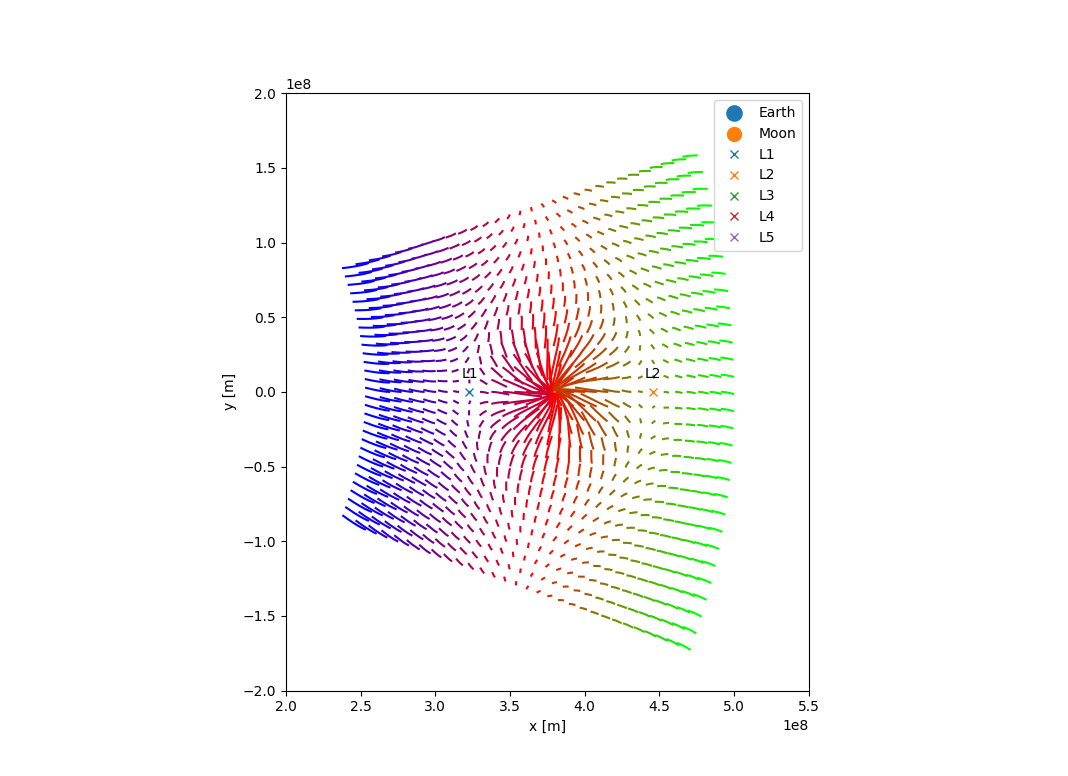
\includegraphics[width=0.9\textwidth]{l12_orbits.png}

    \caption{Trajektorie těles při krátké ($10^5$ s) simulaci v okolí bodů L1 a L2.}
    \label{fig:l12_orbits}
\end{figure}

\subsection{Lagrangův bod L3}

O trochu lépe je na tom se stabilitou bod L3, jak jde vidět na obrázku \ref{fig:l3_orbits}.
Tělesa se správnou vzdáleností od Země se v něm mají docela tendenci držet, i když je to postupně
táhne pryč. Na obrázku jde vidět, že tato stabilita je však velmi výrazně citlivá na vzdálenost od Země
a s větší i menší než správnou vzdáleností tělesa rychle bod opouští.

Ve složce s videi je opět i delší simulace tohoto systému, ve které jde vidět, že většina těles
z tohoto bodu úplně uteče.

\begin{figure}[h!]
    \centering
    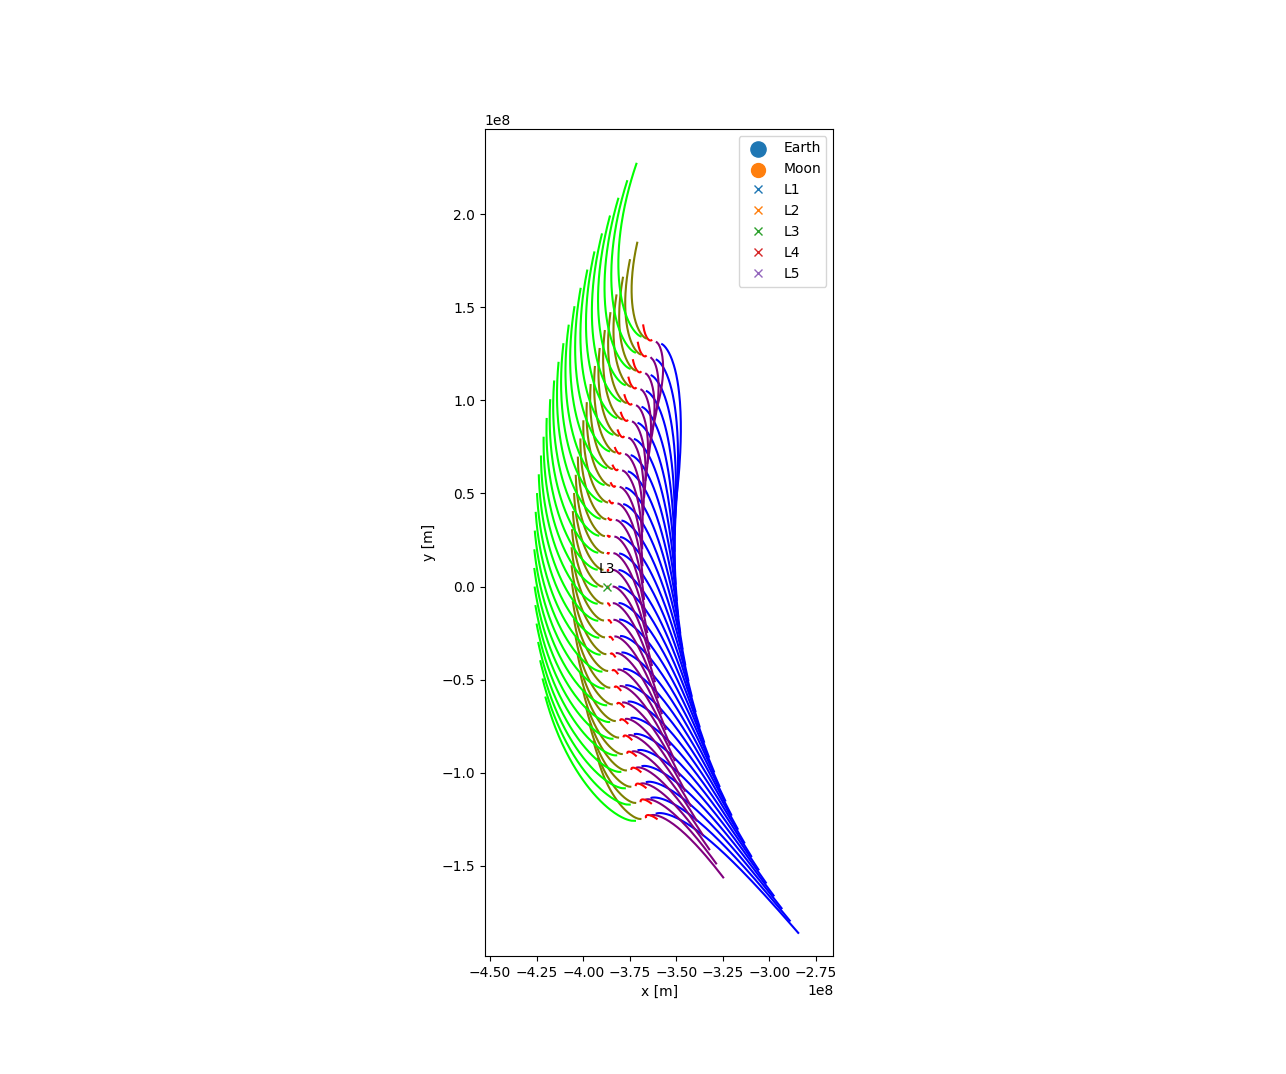
\includegraphics[width=.9\textwidth]{l3_orbits.png}

    \caption{Trajektorie těles při krátké ($10^6$ s) simulaci v okolí bodu L3.}
    \label{fig:l3_orbits}
\end{figure}

\subsection{Lagrangovy body L4 a L5}

Stabilitu bodů L4 a L5 jsem posuzoval rozmístěním těles po celém obvodu systému. Jejich obvodovou 
rychlost jsem přitom nevolil vůči neinerciální soustavě vždy nulovou, ale takovou, aby se tělesa za předpokladu radiálního
pole pohybovaly po kružnici (ve směru oběhu jsem tedy přičítal nebo odčítal korekci v závislosti na vzdálenosti od středu systému).

Počáteční stav simulace a stav po třech letech je vidět na obrázcích \ref{fig:lagrange-25ring-t0} a \ref{fig:lagrange-25ring-t3yr}.
Jak si lze všimnout, zatímco v lagrangových bodech L4 a L5 se vytvořily shluky částic, v ostatních k ničemu takovému nedochází.
Jedině body L4 a L5 jsou tedy pro sondu stabilní i bez přídavných korekcí motorem.

Zajímavé ale je, že se zdá, že oba body v sobě "chytají" jen tělesa, které už v nich nebo v jejich blízkosti na začátku simulace byla
a neuchytí se v nich žádné jiné těleso (to jde vidět hlavně z pravého obrázku - oba Lagrangovy body mají v sobě
jen tělesa velmi podobné barvy). To by však mohlo být i špatnou volbou počátečního rozmístění a rychlostí těles,
na přesnější průzkum bych musel obojí víc randomizovat.

Při porovnání různých časových kroků na obrázcích \ref{fig:lagrange-25ring-comp-t0} a \ref{fig:lagrange-25ring-comp-t3yr}
jde vidět, že po třech letech simulace už většina těles prolétla okolo Země nebo Měsíce a výsledky pro různé časové kroky se tak výrazně
liší. Pro nás je však důležité, že v Lagrangových bodech L4 a L5 toto neplatí, tzn. ve všech třech časových krocích polohy vychází přibližně stejně.
Výsledkům v těchto bodech tedy nejspíš lze věřit.

\begin{figure}[h!]
    \centering
    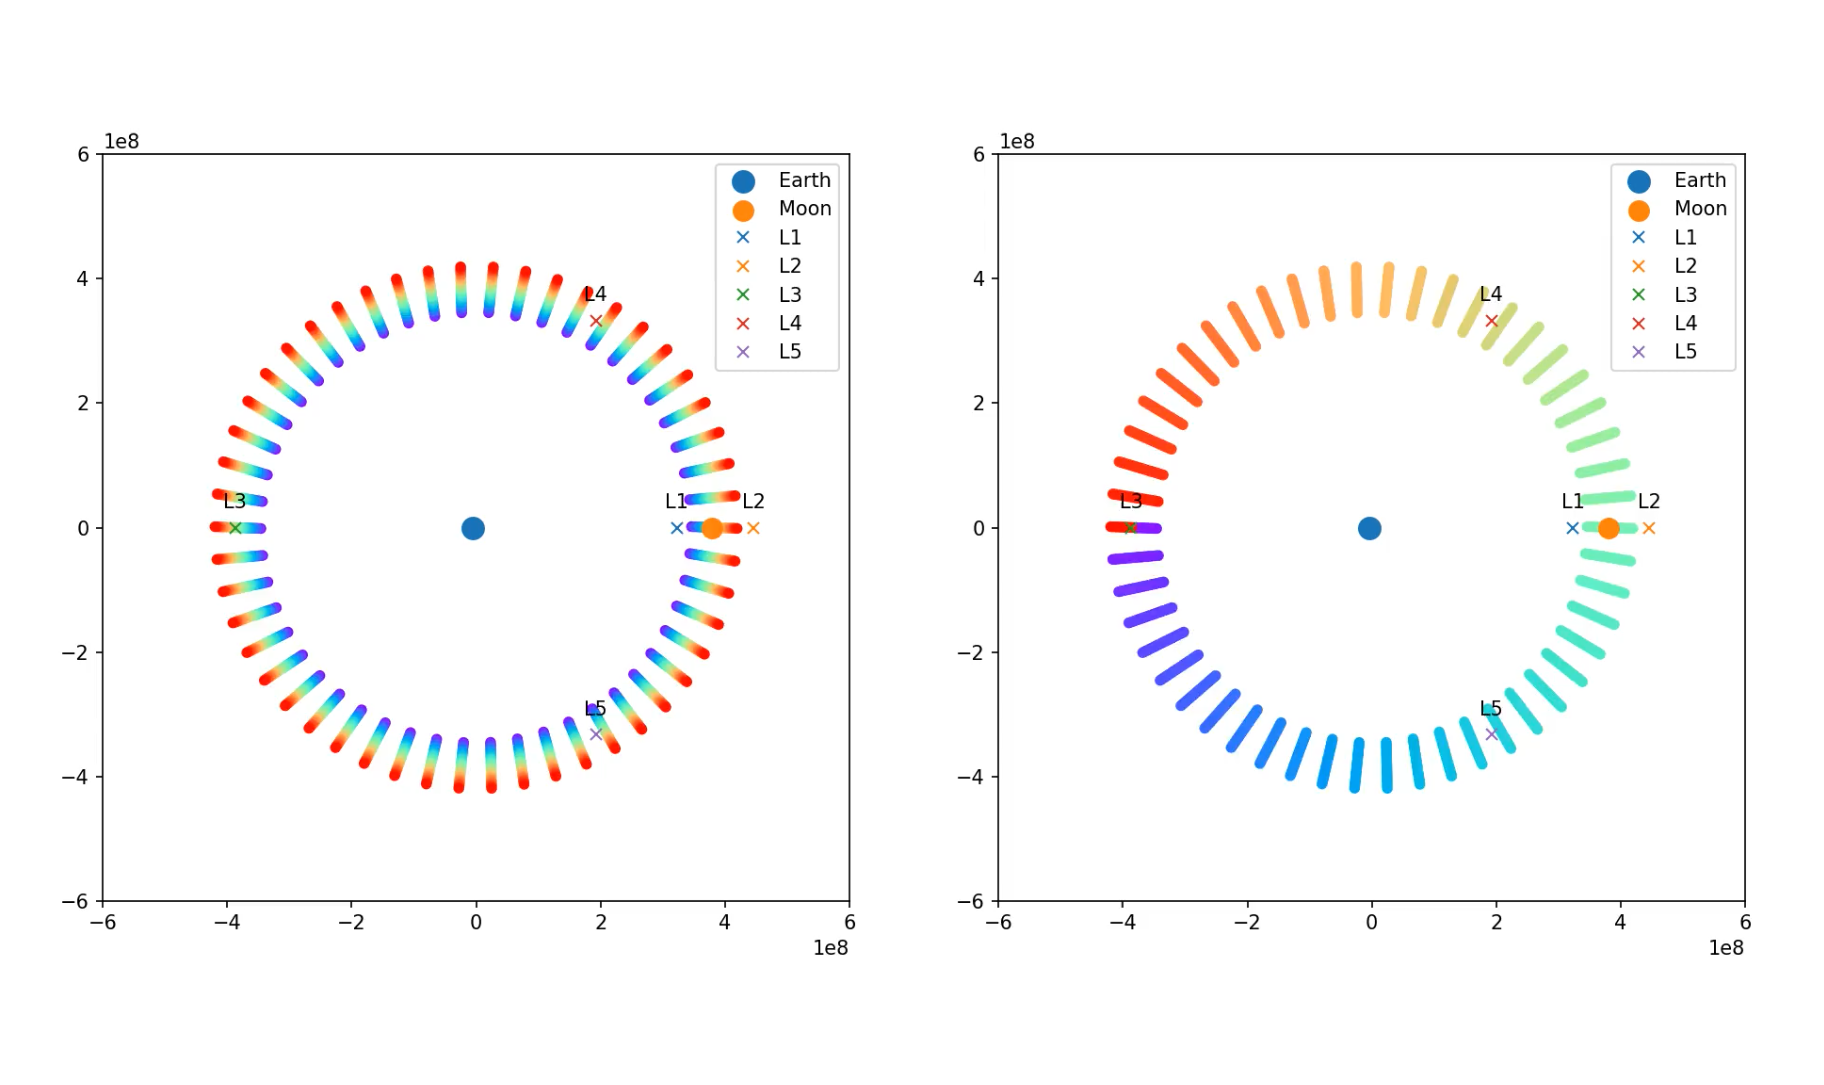
\includegraphics[width=0.9\textwidth]{lagrange-25ring-t0.png}

    \caption{Simulace stability L4 a L5 v nulovém čase.}
    \label{fig:lagrange-25ring-t0}
\end{figure}

\begin{figure}[h!]
    \centering
    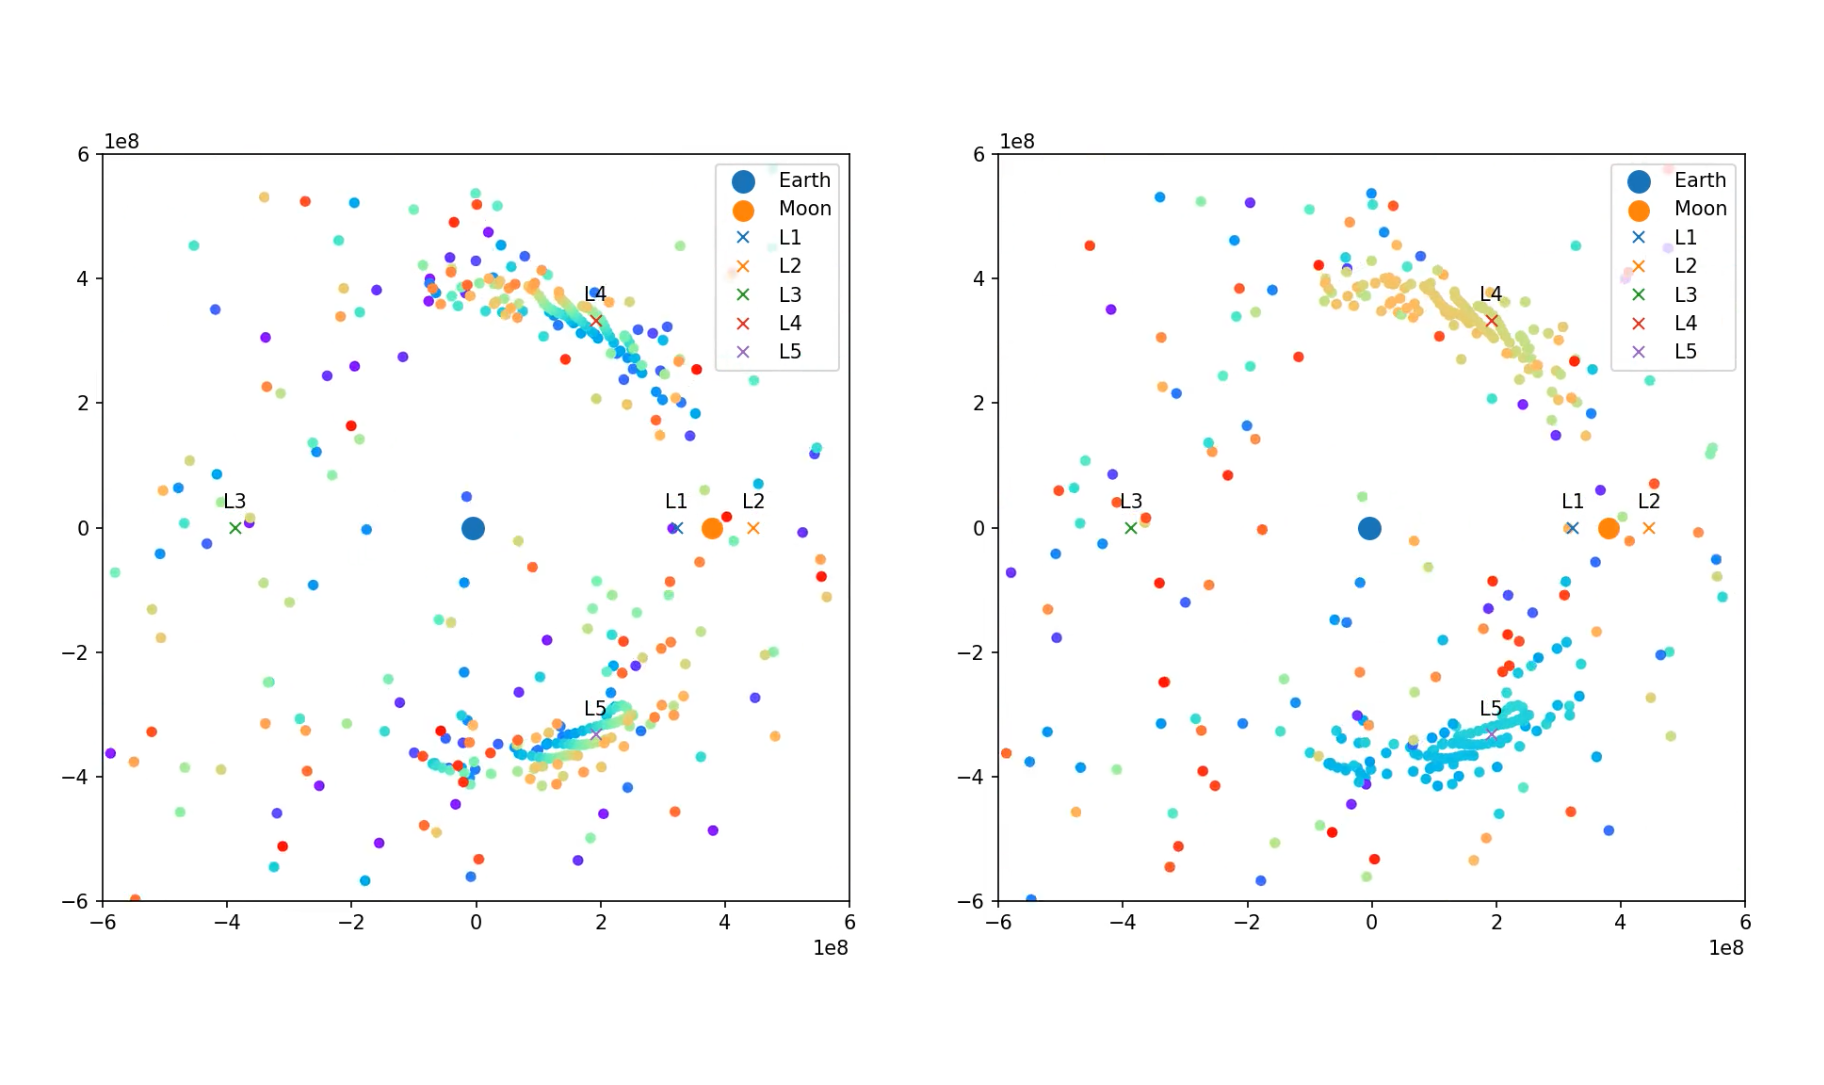
\includegraphics[width=0.9\textwidth]{lagrange-25ring-t3yr.png}

    \caption{Simulace stability L4 a L5 po třech letech.}
    \label{fig:lagrange-25ring-t3yr}
\end{figure}

\begin{figure}[h!]
    \centering
    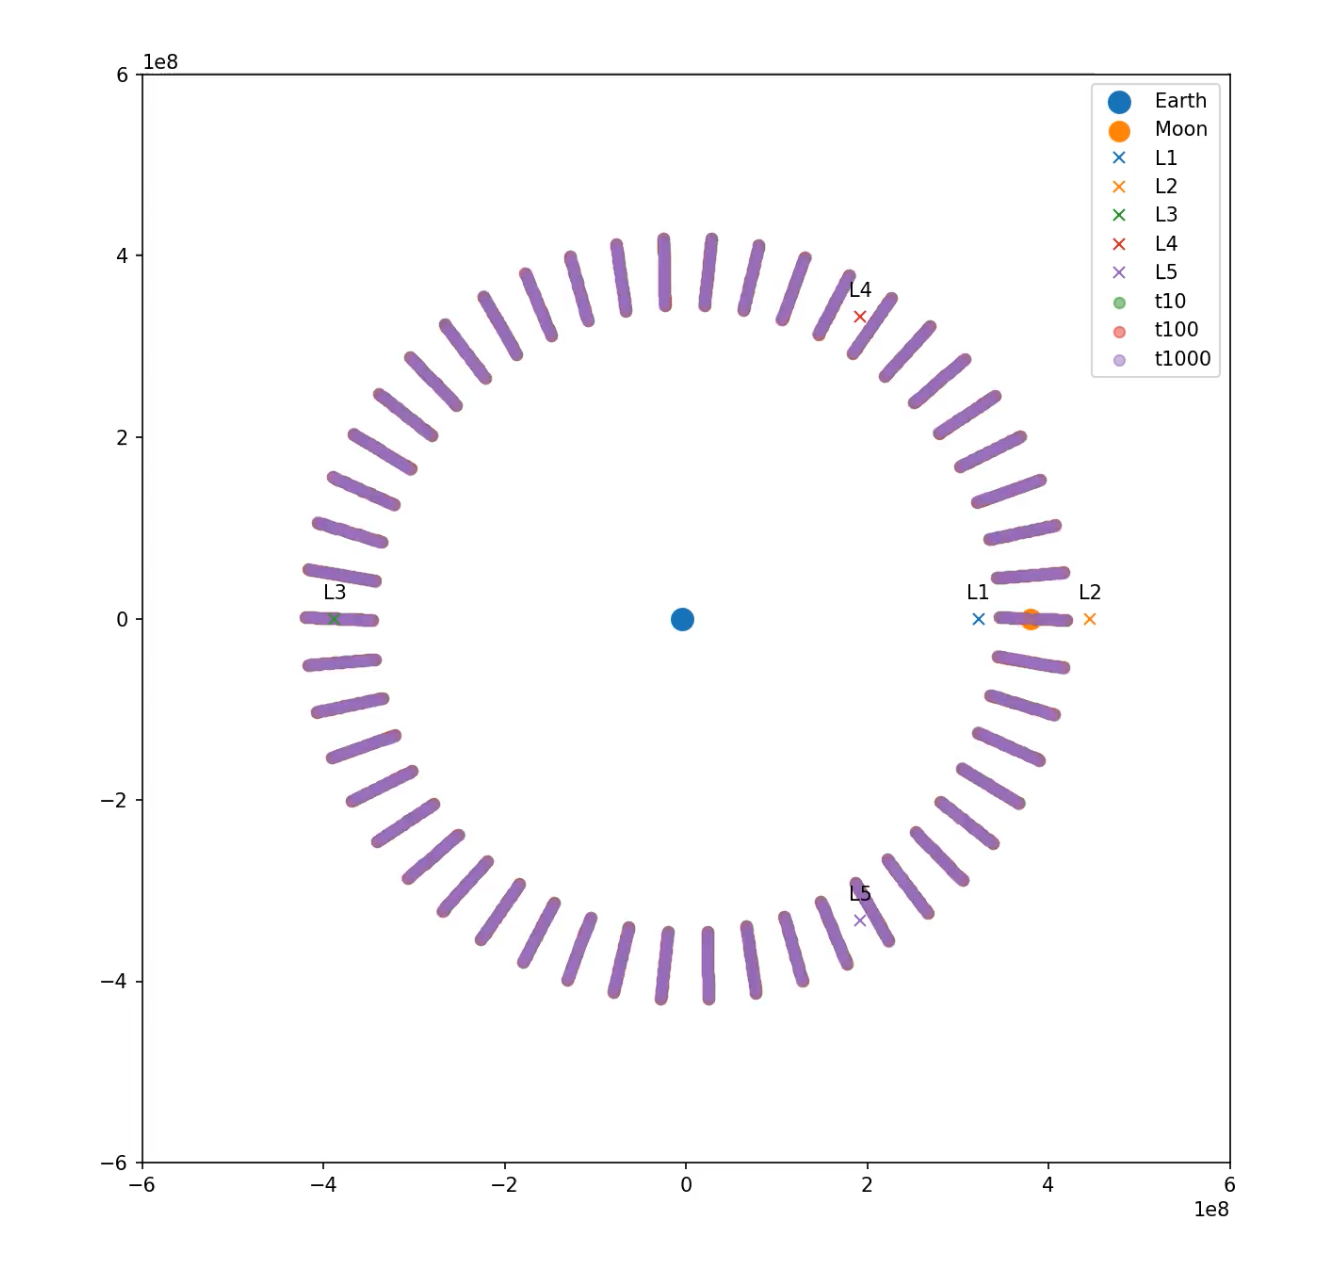
\includegraphics[width=0.6\textwidth]{lagrange-25ring-comp-t0.png}

    \caption{Simulace stability L4 a L5 v nulovém čase - porovnání časových kroků 10s, 100s a 1000s.}
    \label{fig:lagrange-25ring-comp-t0}
\end{figure}

\begin{figure}[h!]
    \centering
    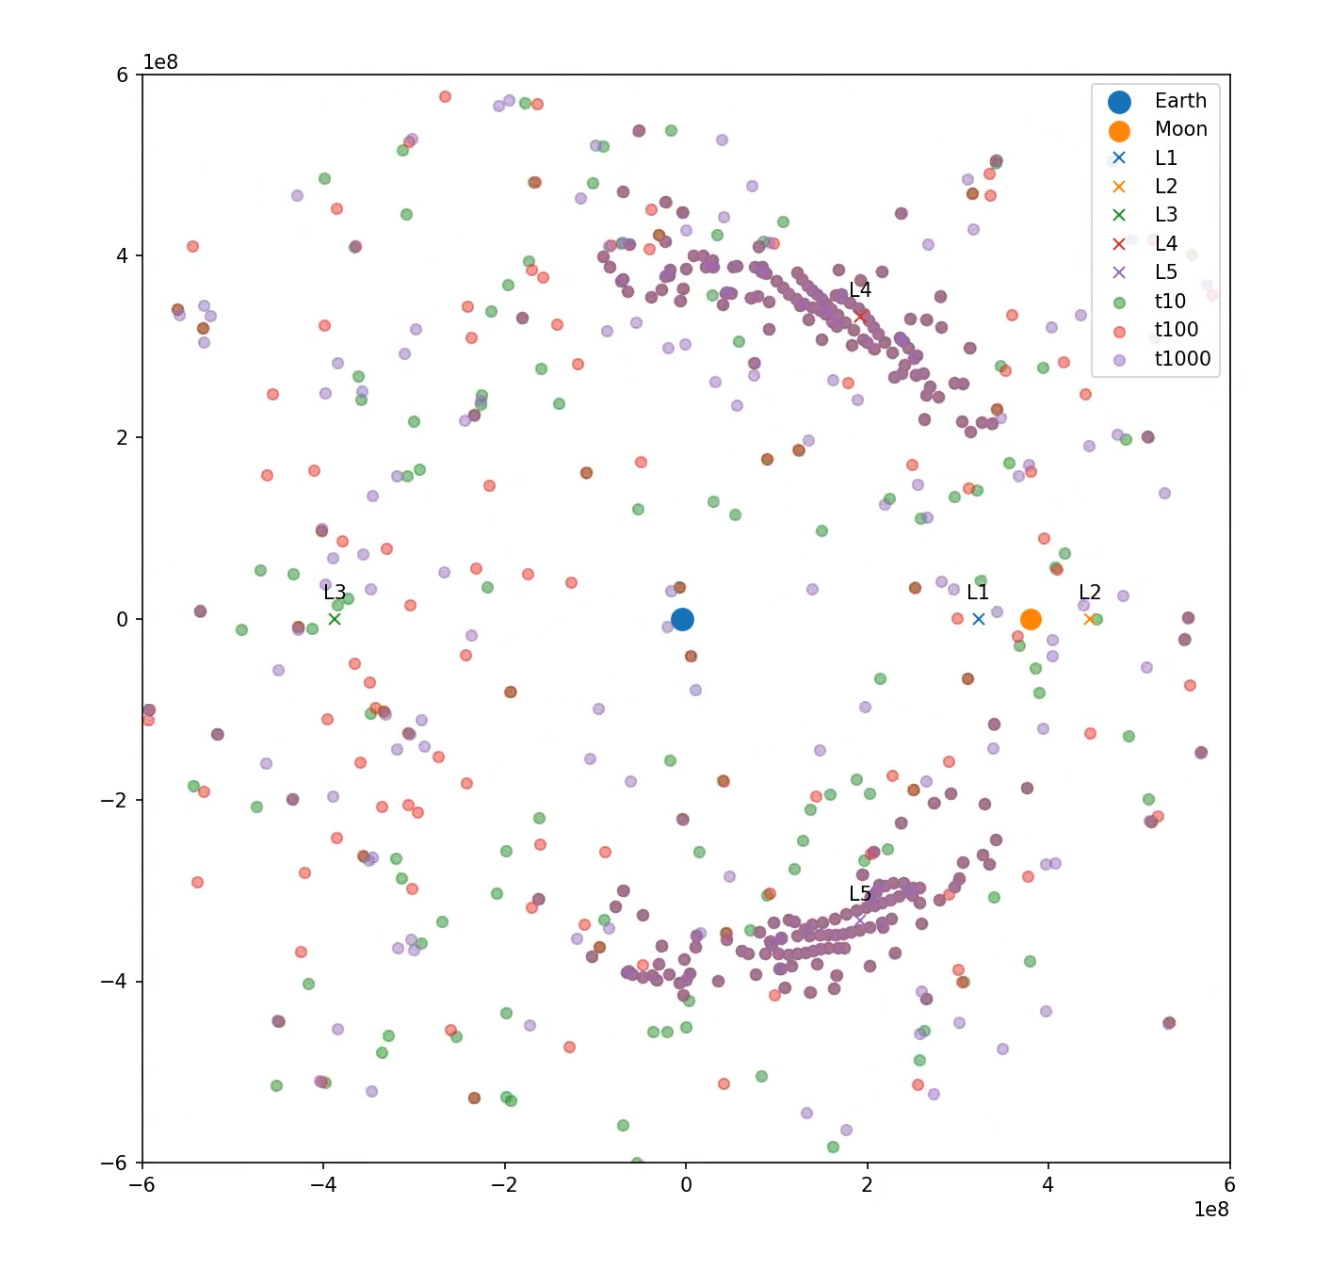
\includegraphics[width=0.6\textwidth]{lagrange-25ring-comp-t3yr.png}

    \caption{Simulace stability L4 a L5 po třech letech - porovnání časových kroků 10s, 100s a 1000s.}
    \label{fig:lagrange-25ring-comp-t3yr}
\end{figure}

\end{document}